%----------------------------------------------------------------------------------------
% METADATA BLOCK (YAML)  — see inbox/README.md
%----------------------------------------------------------------------------------------
% uid: ""
% school: "lycee"
% level: "3eme"
% section: "Economie et Gestion"
% chapter: "Statistiques"
% title: "Prix et demande"
% difficulty: "Facile"
% tags: ["statistiques", "serie-double", "nuage-de-points", "point-moyen"]
% provenance: "own"
% batch: "2026-11-19-3eco-statistiques-n5"
%----------------------------------------------------------------------------------------

\newcommand{\R}{\mathbb{R}}
\newcommand{\vect}[1]{\overrightarrow{#1}}

% ---STATEMENT---
Une entreprise a relevé la quantité demandée $y$ (en centaines d'unités) d'un produit selon son prix de vente $x$ (en dinars) :
\begin{center}
\begin{tabular}{|l|c|c|c|c|c|c|}\hline
Prix $x_i$ & $2$ & $3$ & $4$ & $5$ & $6$ & $7$ \\\hline
Demande $y_i$ & $52$ & $46$ & $42$ & $36$ & $30$ & $28$ \\\hline
\end{tabular}\end{center}
\begin{enumerate}
  \item Représenter le nuage de points de la série $(x_i\,;y_i)$ dans un repère orthogonal.
  \item Calculer les coordonnées du point moyen $G$ et le placer.
  \item Décrire l'allure du nuage. Comment varie la demande quand le prix augmente ?
\end{enumerate}

% ---SOLUTION---
\begin{enumerate}[itemsep=14pt]
  \item
  \begin{center}
% alt: Nuage de six points décroissant (prix, demande) et point moyen G(4,5 ; 39).
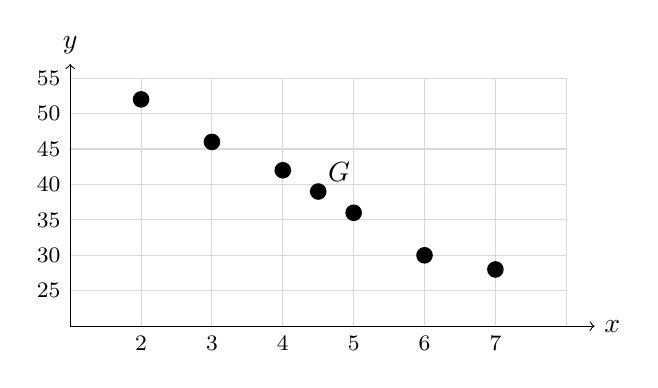
\begin{tikzpicture}[x=0.9cm,y=0.09cm]
    \draw[gray!30] (1,20) grid[xstep=1,ystep=5] (8,55);
    \draw[->] (1,20)--(8.4,20) node[right]{$x$};
    \draw[->] (1,20)--(1,57) node[above]{$y$};
    \foreach \x in {2,...,7} \node[below] at (\x,20) {\footnotesize\x};
    \foreach \y in {25,30,...,55} \node[left] at (1,\y) {\footnotesize\y};
    \foreach \x/\y in {2/52,3/46,4/42,5/36,6/30,7/28} \fill (\x,\y) circle (3pt);
    \fill[black] (4.5,39) circle (3pt) node[above right]{$G$};
  \end{tikzpicture}
  \end{center}
  (L'axe des ordonnées commence à $20$ pour mieux voir le nuage.)

  \item
  \begin{prop}[Point moyen]
  Le point moyen du nuage est \ib{$G(\overline x\,;\overline y)$}.
  \end{prop}
  \[\overline x=\dfrac{2+3+4+5+6+7}{6}=\dfrac{27}{6}=4{,}5\qquad\overline y=\dfrac{52+46+42+36+30+28}{6}=\dfrac{234}{6}=39\]
  \[G(4{,}5\,;39)\]

  \item Les points sont presque alignés sur une droite qui \textbf{descend} : quand le prix augmente, la demande diminue (d'environ $5$ centaines d'unités par dinar).
\end{enumerate}
